\documentclass[crop,tikz,border=1px]{standalone}

\usepackage{color}
\newcommand{\red}[1]{\textcolor{red}{#1}}

\usetikzlibrary{arrows,positioning,scopes,automata}

\begin{document}
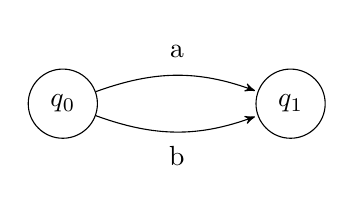
\begin{tikzpicture}[->,>=stealth',shorten >=1pt,auto,node
  distance=2cm,inner sep=2pt,minimum size=.6cm,
  mystate/.style={state,text centered}]

  \node[mystate] (q0) {\(q_0\)};
  \node[mystate] (q1) [right=of q0] {\(q_1\)};

  \path (q0) edge [bend left=20] node [above] {a} (q1)
        (q0) edge [bend right=20] node [below] {b} (q1);

\end{tikzpicture}
\end{document}
